\section{Evaluation}

In this section, we will evaluate our solution and implementation in terms of security and performance. 

\subsection{Security Analysis}

Our adversarial model is that we assume the adversary has the capability to upload malicious logic to the PLC that will generate erroneous outputs or further compromise the entire PLC. 

In addition, we assume that the logging mechanism is working properly until a certain point after the compromise initiates. In other words, we assume there exist a time window that the attacker has initiated the intrusion, but the logging is still working properly. The overall timeline can be illustrated as Figure.~\ref{fig:timeline}. 

\begin{figure*}[h]
  \centering
    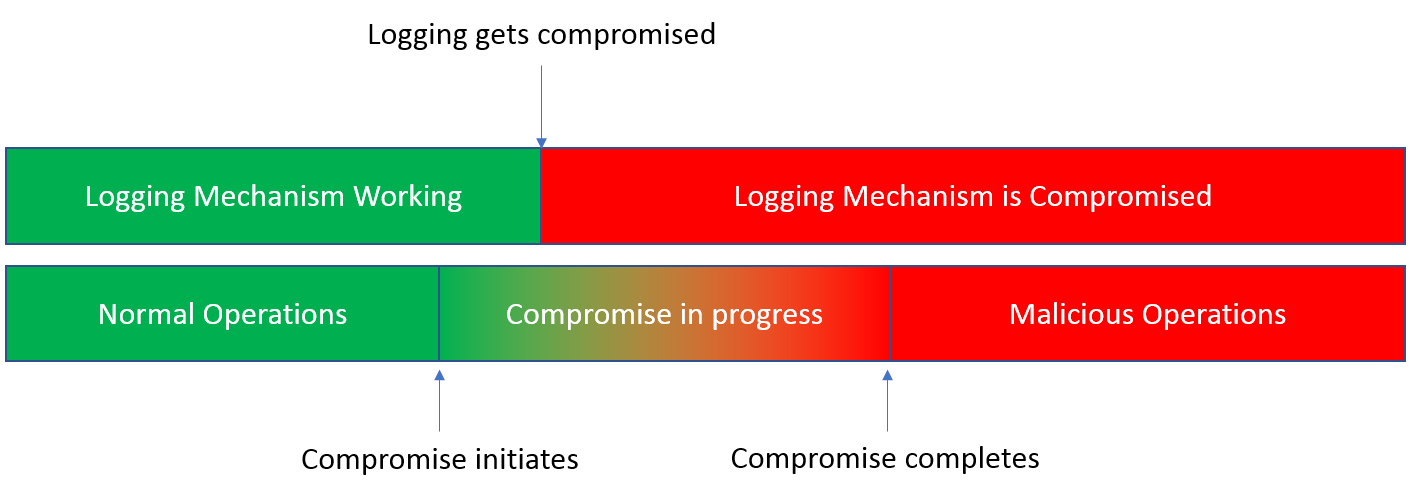
\includegraphics[width=\textwidth]{figs/timeline}
    \caption{Time line of one compromise.}
    \label{fig:timeline}
\end{figure*}
   
\subsection{Performance Overhead}